% Created 2023-04-12 Wed 14:17
% Intended LaTeX compiler: pdflatex
% =================================BASE====================================%
\documentclass{article}
\usepackage[left=2cm,right=2cm,top=2cm,bottom=2cm]{geometry} % Marges
\usepackage[utf8]{inputenc} % Important pour symboles Francophones, é,à,etc.
\usepackage[T1]{fontenc} % Nécessaire avec FrenchBabel

\usepackage{natbib} % Bibliographie
\bibliographystyle{abbrvnat}
\usepackage[french, american]{babel} % Environnements en Français.


\usepackage{amsmath, amssymb, amsthm} % Symb. math. (Mathmode+Textmode) + Beaux théorèmes.

\usepackage{mathtools, cancel} % Utilisation de boîtes \boxed{} + \cancelto{}{}
\usepackage{graphicx, wrapfig} % Géstion des figures.
\usepackage{hyperref} % Permettre l'utilisation d'hyperliens.
\usepackage{color} % Permettre l'utilisation des couleurs.
\usepackage[dvipsnames]{xcolor} % Couleurs avancées.
\usepackage{titling} % Donne accès à \theauthor, \thetitle, \thedate

% >>> Physique >>>
\usepackage{physics} % Meilleur package pour physicien. 
\usepackage{pxfonts} % Rajoute PLEIN de symboles mathématiques, dont les intégrales doubles et triples
% <<< Physique <<<

\usepackage{lipsum} % For fun
\usepackage{tikz} % Realisation de figures TIKZ.
\usepackage{empheq} % Boite autour de MULTIPLE équations
% =================================BASE====================================%



% ================================SETTINGS=================================%
%%% - Pas d'indentation en début de paragraphe :
\setlength\parindent{0pt} 
%%% - Couleurs de hyperliens :
\hypersetup{colorlinks,urlcolor=cyan,citecolor=blue,linkcolor=teal}
%%% - Numéros d'équations suivent les sections :
\numberwithin{equation}{section} 
%%% - Les « captions » sont en italique :
\usepackage[textfont = it]{caption} 
% ================================SETTINGS=================================%



% ==============================NEWCOMMANDS================================%
% Degrés Celsius :
\newcommand{\celsius}{${}^\circ$ C} % \degrée Celsius : Pas mal plus simple qu'utilise le package gensymb qui plante avec tout...

% Vecteurs de base :
\newcommand{\nvf}{\hat{\vb{n}}}
\newcommand{\ivf}{\vb{\hat{i}}}
\newcommand{\jvf}{\hat{\vb{j}}}
\newcommand{\kvf}{\hat{\vb{k}}}

% Empty frac-Box
\newcommand{\bigno}{\vphantom{\qty(\frac{d}{q})}}

\newcommand{\tpsi}{\tilde{\psi}}
% ==============================NEWCOMMANDS================================%



% =================================ENTÊTE==================================%
\usepackage{fancyhdr}
\pagestyle{fancy}
\setlength{\headheight}{13pt}

\fancyhead[L]{$\cdot$\ \nouppercase{\leftmark} }
\fancyhead[R]{C.-É. Lizotte\ $\cdot$}
\fancyfoot[C]{$\cdot$ \thepage\ $\cdot$}
% =================================ENTÊTE==================================%
\author{Charles-Édouard Lizotte}
\date{31/03/2023}
\title{Rapport hebdomadaire -- McGill\\\medskip
\large Semaine du 27 mars 2023}
\hypersetup{
 pdfauthor={Charles-Édouard Lizotte},
 pdftitle={Rapport hebdomadaire -- McGill},
 pdfkeywords={},
 pdfsubject={},
 pdfcreator={Emacs 27.1 (Org mode 9.6.2)}, 
 pdflang={English}}
\begin{document}

\maketitle
\tableofcontents



\section{{\bfseries\sffamily DONE} Run du modèle multicouches}
\label{sec:orgef051e7}
\subsection{Mise en contexte et paramètres}
\label{sec:org414c76c}
Au cours de la fin de semaine du 25 au 26, j'ai testé le modèle à 3 couches pour une période de 5 ans.
Le modèle a terminé sa course sans accrochage avec les paramètres du tableau \ref{tab:orgd099e41}.

\begin{table}[htbp]
\caption{\label{tab:orgd099e41}Valeur des différents paramètres de l'expérience de \cite{chen_2021}, mais à 3 couches.}
\centering
\begin{tabular}{lll}
\hline
\hline
Paramètres & Symbole & Valeur\\[0pt]
\hline
Taille du domaine & L\textsubscript{x} = L\textsubscript{y} & 2000 km\\[0pt]
Pas de temps & \(\Delta\) t & 360 s\\[0pt]
Paramètre de Coriolis & f & 7\texttimes{}10\textsuperscript{-5} s\textsuperscript{-1}\\[0pt]
Amplitude du vent & \(\tau\)\textsubscript{atm} & 0.1 N m\textsuperscript{-2}\\[0pt]
Coefficient de viscosité biharmonique & A\textsubscript{bh} & dx\textsuperscript{4} \texttimes{}10\textsuperscript{-5} s\textsuperscript{-1}\\[0pt]
Coefficient de frottement au fond & r\textsubscript{drag} & 10\textsuperscript{-7} s\textsuperscript{-1}\\[0pt]
Coefficient dissipation du Laplacien inverse & r\textsubscript{InvLap} & (2\(\pi\)/L\textsubscript{y})\textsuperscript{2} \texttimes{} 10\textsuperscript{-6} s\textsuperscript{-1}\\[0pt]
Épaisseur de la couche en surface & H\textsubscript{1} & 1000 m\\[0pt]
Épaisseur de la seconde couche & H\textsubscript{2} & 1000 m\\[0pt]
Épaisseur de la couche au fond & H\textsubscript{3} & 2000 m\\[0pt]
Densité de l'eau (première couche) & \(\rho\)\textsubscript{1} & 1.0000 kg/m\textsuperscript{3}\\[0pt]
Densité de l'eau (seconde couche) & \(\rho\)\textsubscript{2} & 1.0016 kg/m\textsuperscript{3}\\[0pt]
Densité de l'eau (troisième couche) & \(\rho\)\textsubscript{3} & 1.0024 kg/m\textsuperscript{3}\\[0pt]
Vitesse des ondes internes (semi-obsolète) & c\textsubscript{bc} & 2 ms\textsuperscript{-1}\\[0pt]
Gravité réduite (seconde couche) & g\textsubscript{2}' & 8 \texttimes{} 10\textsuperscript{-2} m/s\textsuperscript{2}\\[0pt]
Gravité réduite (troisième couche) & g\textsubscript{3}' & 6 \texttimes{} 10\textsuperscript{-3} m/s\textsuperscript{2}\\[0pt]
\hline
\hline
\end{tabular}
\end{table}

\subsection{Quelques résultats encourageants}
\label{sec:org5f66570}
Avant tout, j'avais modifié les sous-routine de \emph{output} pour qu'on puisse avoir quelque chose à observer.
En fin de semaine le modèle semblait de bien fonctionner, mais en observant les output, j'ai remarqué qu'il n'y avait aucune production barocline.
Je croyais que mon vent n'était pas assez fort, mais c'était plutôt une erreur de \emph{timestep}.
Le deuxième \emph{RHS} mettait à jours eta(2) et non eta(3), \emph{rookie mistake}.
Après avoir détecté l'erreur avec David, j'ai donc relancé l'expérience ce mercredi en soirée avec les paramètres cités dans le tableau \ref{tab:orgd099e41}.
Après quelques essais et erreurs, les valeurs de densité \(\rho_k\) ont été choisies dans le but de mimiquer les gravité réduites trouvées à partir de la vitesse des ondes baroclines \(c_{bc}\), soit
\begin{equation}
g_k' = \qty(\frac{H}{H_k\cdot H_{k-1}}) \ c_{bc}^2.
\end{equation}
Des diagrames de Hovmoller pour les résultats de la \emph{run} de mercredi devraient se retrouver en annexe.

\section{{\bfseries\sffamily DONE} Retrouver les vorticités barotropes et baroclines}
\label{sec:org241782b}
\subsection{\textbf{Rappel théorique} :  La mécanique des ondes de Rossby dans une couche}
\label{sec:orgf103ec3}
Dans cette sous-section, nous allons développer les équations de vorticité quasi-géostrophique de sorte à retrouver la relation de dispersion des ondes de Rossby.
Comme le développement mathématique des ondes de Rossby est intrinsèquement relié aux modes barotrope et baroclines, nous allons revisiter le concept en quelques lignes.\bigskip

Comme nous l'avons vu dans le dernier \href{rapport-2023-03-24.org}{rapport}, la vorticité potentielle QG est donnée par l'expression
\begin{equation}
\label{eq:org7797a3f}
q = \zeta + \beta - \frac{f_0}{H} \eta' = \laplacian \psi + \beta y - \frac{1}{L_d^2} \psi,
\hspace{0.5cm}\text{où}\hspace{0.5cm}
\dv{q}{t} = \pdv{q}{t} + \vb{u} \cdot \gradient q = \pdv{q}{t} + J(\psi,q) =  0.
\end{equation}
On recherche un type d'onde à méso-échelle, donc posons que la circulation à l'étude est vraiment plus petite que le rayon de déformation, de sorte que \(L_d \rightarrow \infty\) et \(q \rightarrow \zeta + \beta y\).
Appliquons cette nouvelle définition dans l'équation d'évolution de \(q\) (eq. \ref{eq:org7797a3f}) pour retrouver
\begin{equation}
\label{eq:org3fd27c7}
\pdv{\zeta}{t} + \underbrace{\pdv{(\beta y)}{t}}_{=0} + \vb{u}\cdot \gradient \zeta + \underbrace{\vb{u} \cdot \gradient(\beta y)\bigno}_{ =\beta v}
= \boxed{
\pdv{\zeta}{t} + \vb{u}\cdot\gradient\zeta  + \beta v = 0
}
\end{equation}

À partir d'ici, il est souhaitable de \textbf{linéariser} l'équation d'évolution de la QGPV (\ref{eq:org3fd27c7}) en posant un courant moyen  en \emph{x} en arrière plan, (\emph{background flow}), de sorte que \(\psi = \bar{\psi}(y) + \psi'(x,y,t)\) où \(\bar{\psi}(y)=-\bar{u}y\).
\begin{align}
\label{eq:org80a212a}
&\pdv{t} \laplacian \psi' + \underbrace{\bar{u}\cdot \gradient (\laplacian \bar{\psi}) }_{=0}
+ \bar{u}\cdot \gradient (\laplacian \psi')
+ \underbrace{u'\cdot \gradient (\laplacian \bar{\psi}) }_{=0}
+ \beta \pdv{\psi'}{x} = 0,\nonumber \\
%
&\pdv{t} \laplacian \psi' + \bar{u}\pdv{x} (\laplacian \psi') + \beta \pdv{\psi'}{x} = 0.
\end{align}
\textbf{N.B.} La proposition \(\bar{\psi} = -\bar{u} y\) est assez consistante avec notre présomption que que \(L_d\) est très grand. \bigskip

Par coutume, il est de mise de poser des solutions ondulantes de la forme
\begin{equation}
\psi' = \exp{i(kx + ly -\omega t)},
\end{equation}
dans (\ref{eq:org80a212a}) ce qui nous amènera à l'équation de dispersion pour les ondes des Rossby à une couche, soit
\begin{equation}
(i)^2 K^2(-i\omega) + (i)^3\bar{u} k K^2 + i \beta k = 0
\hspace{0.8cm}\Longrightarrow\hspace{0.8cm}
\boxed{\omega = k \ \qty(\bar{u} - \frac{\beta}{K^2}),}
\end{equation}
où \(K^2 \equiv k^2 + l^2\).\bigskip

Finalement, les \textbf{vitesse de groupe} et \textbf{de phase} sont respectivement données par
\begin{align}
\text{Phase}\hspace{1cm} & c^x_p = \frac{\omega}{k} = \bar{u} - \frac{\beta}{K^2}, \hspace{2.4cm} c^y_p = \frac{\omega}{l} = \bar{u} \frac{k}{l} - \frac{\beta k}{K^2 l},\\
\text{Groupe}\hspace{0.8cm} &c^x_g = \pdv{\omega}{k} = \frac{\beta(k^2-l^2)}{(k^2 + l^2)} \hspace{2cm} c^y_g = \pdv{\omega}{l} = \frac{2\beta k l}{(k^2 + l^2)^2}.
\end{align}

\subsection{Interprétation physique des ondes de Rossy}
\label{sec:orgea91fbb}
Le livre de \cite{vallis_2006} offre une interprétation physique élégante du méchanisme de rappel des ondes de Rossby.
En subissant des perturbations zonales, les parcelles de fluides vont vouloir conserver leur vorticité.
Ce faisant, elle transforment de la vorticité planétaire en vorticité relative et se mettent en rotation.
Ceci aura tendance à advecter la parcelle vers l'ouest, comme décrit dans l'image \ref{fig:orgc67d2cc}.

\begin{figure}[htbp]
\centering
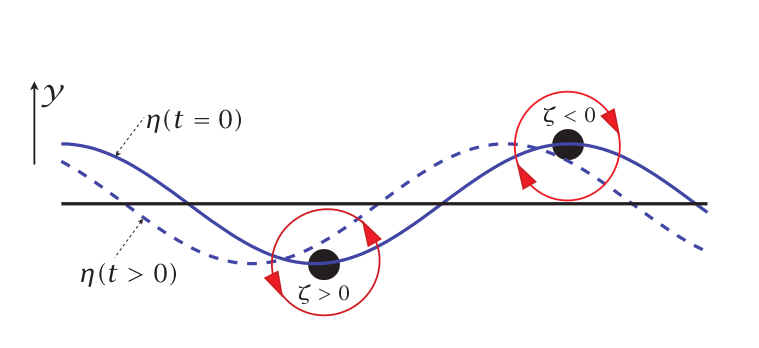
\includegraphics[width=.9\linewidth]{figures/vallis/vallis_rossby_simplification.png}
\caption{\label{fig:orgc67d2cc}Figure tirée du Vallis décrivant le comportement des parcelles de fluide à l'équateur.}
\end{figure}

\subsection{Description du système QG à \textbf{deux niveaux}}
\label{sec:org7197869}

Toujours en partant des équation QG en milieu continu, il est possible de définir l'équation de vorticité quasi-géostrophique à \textbf{deux ou plusieurs niveaux}.
Nous utiliserons ici la technique des différences finies pour discrétiser les équations continues et trouver un modèle à deux couches, un cas spécial aussi appelé modèle de Philips (\cite{vallis_2006}).\bigskip

Premièrement, la QGPV en milieu continu est donnée par 
\begin{equation}
q = \zeta + f + \pdv{z} \qty(\frac{f_0 b'}{N^2}).
\end{equation}

La \textbf{flottabilité} peut être décrite comme une dérivée verticale de la fonction de courant entre les deux niveaux (Voir figure \ref{org66eb6a6}).
Nous approximerons cette dérivée par une différence finie, de sorte que
\begin{equation}
b' = f_0\pdv{\psi}{z} \sim f_0 \qty(\frac{\Delta \psi}{\Delta z}) = \frac{f_0 (\psi_1 - \psi_2)}{H/2}.
\end{equation}

\begin{wrapfigure}[15]{r}{0.5\textwidth}
\centering
\begin{tikzpicture}[scale = 1.7]
%%% Fill boxes
\fill [blue!14] (0,0.0) rectangle (3,2.5);
\fill [blue!8]  (0,2.5) rectangle (3,4.0);
% Hard lines 
\draw[thick]  (0,0) -- (3,0);
\draw[dashed] (0,2.5) -- (3,2.5);
\draw[thick]  (0,4) -- (3,4);
%%% Psi lines
\node at (1.25,3.25) (psi1) {$\psi_1,q_1$};
\node at (1.25,1.25) (psi2) {$\psi_2,q_2$};
\draw[dotted, thin] (0,3.25) -- (psi1) -- (3,3.25);
\draw[dotted, thin] (0,1.25) -- (psi2) -- (3,1.25);
%&& Lenght H mesures
\node at (-0.25,3.25) (h1) {$\mathrm{H}_1$};
\node at (-0.25,1.25) (h2) {$\mathrm{H}_2$};
%
\draw[>=stealth, ->|] (h1) -- (-0.25,2.5)  ;
\draw[>=stealth, ->|] (h1) -- (-0.25,4)    ;
%
\draw[>=stealth, ->] (h2) -- (-0.25,2.5)   ;
\draw[>=stealth, ->] (h2) -- (-0.25,0)     ;
%
%%% Half lenght
\node at (2.65,3.625) (h12) {$\mathrm{H}_1/2$};
\node at (2.65,0.625) (h22) {$\mathrm{H}_2/2$};
\draw[>=stealth, thin, |<->|] (2.3,3.25) -- (2.3,4);
\draw[>=stealth, thin, |<->|] (2.3,0) -- (2.3,1.25);
%%% Flottabilité
\node at (3.25,2.5) (b) {$b'$};
\draw[>=stealth, ->|] (b) -- (3.25,1.25);
\draw[>=stealth, ->|] (b) -- (3.25, 3.25);
%
\end{tikzpicture}
\caption{\label{org66eb6a6}Schéma conceptuel du modèle QG à deux \textbf{niveaux}. Les fonctions de courant et les vorticité potentielles}
\end{wrapfigure}

Les vorticités potentielles des deux niveaux sont ainsi exprimées par
\begin{subequations}
\label{eq:org072b54c}
\begin{equation}
q_1 = \zeta_1 + f + \frac{2 f_0^2}{N^2 H_1 H} (\psi_2 - \psi_1);
\end{equation}
\begin{equation}
q_2 = \zeta_2 + f + \frac{2 f_0^2}{N^2 H_2 H} (\psi_1 - \psi_2).
\end{equation}
\end{subequations}
et les équations de conservation sont -- comme à l'habitude -- données par
\begin{equation}
\pdv{q_i}{t} + J (\psi_i,q_i) = 0,
\hspace{0.5cm} \text{et} \hspace{0.5cm}
i \in \qty{1,2}.
\end{equation}
\textbf{N.B.} Le \(J(\psi,...)\) décrit le Jacobien entre la fonction de courant et une autre fonction.
\vspace{2cm}

\subsection{Connection entre les système à \textbf{deux niveaux} celui à \textbf{deux couches}}
\label{sec:org31c7876}
On se doute bien qu'il existe un lien entre les équations à deux couches et les équations à deux niveaux, en effet
\begin{equation}  
N^2 = \pdv{\hat{b}}{z}; \hspace{1.5cm} b = \frac{-g\delta \rho}{\rho_0},
\end{equation}
donc si l'on approxime l'écart de densité et d'échelle verticale comme étant une différence finie, on arrive à
\begin{equation}
N^2 = \frac{g}{f_0} \frac{\rho_1 - \rho_2}{H_2} = \frac{g_2'}{H/2}.
\end{equation}

Par conséquent, les équations \ref{eq:org072b54c} deviennent
\begin{align}
&q_1 = \zeta_1 + f + \frac{f_0^2}{g_2' H_1} (\psi_2 - \psi_1);
&q_2 = \zeta_2 + f + \frac{f_0^2}{g_2' H_2} (\psi_1 - \psi_2),
\end{align}
soit les équations de QGPV à deux couches.
Pour citer \cite[p.195]{vallis_2006} :
\begin{quote}
\textit{« Similarly, a multilayered system with n-layers is equivalent to a finite difference representation with n-levels »}
\end{quote}

Donc à \(nz\) couches, on peut généraliser \(\Delta z_k = (H_k + H_{k-1})/2\), de sorte que
\begin{equation}
\label{eq:org0f0a3a1}
q_k = \zeta_k + f_k + \frac{f_0^2}{g_k' H_k}(\psi_{k-1} - \psi_k) - \frac{f_0^2}{g_{k+1}' H_k}(\psi_k - \psi_{k+1}).
\end{equation}
En conclusion, on peut dicrétiser les équations en milieu continu à l'aide de la méthode des différences finies (sinon, ça serait difficile de faire de la numérique), tout en se permettant d'avoir une résolution horizontale de seulement deux couches.
Le but de cet exercice était prinipalement de se convaincre qu'on peut passer d'un milieu continu sans se mettre dans le pétrin.
Dans la section suivante, nous développerons l'équation d'évolution de la QGPV linéarisée, mais pour \(L_d \not = \infty\).

\subsection{Description des modes barotrope et baroclines}
\label{sec:orgbae2100}
Précédemment, nous avons utilisé l'équation d'évolution de la QGPV pour trouver la relation de dispersion des ondes de Rossby, cette équation était donnée par
\begin{equation}
\label{eq:org55c791c}
\pdv{t} \Bigg[ \laplacian \psi' + \frac{1}{\tilde{\rho}(z)}\pdv{z}\qty(\frac{f_0}{N^2}\pdv{\psi'}{z}) \Bigg] + \beta \pdv{\psi'}{x} = 0.
\end{equation}
Ensuite, nous avions linéarisé l'équation précédente autour d'un courant moyen en \emph{x} en assumant que \(L_d \rightarrow \infty\).
Ici, nous allons exactement réaliser l'inverse en posant une solution oscillante de la forme
\begin{equation}
\psi'(x,,y,z,t) = \Re \tpsi(z) \exp{ i(kx + ky - \omega t)},
\end{equation}
dans l'équation \ref{eq:org55c791c}.\bigskip

On arrive à
\begin{equation}
\label{eq:org0b2ff9f}
\omega\ \Bigg[ - K^2 \cdot \tpsi(z) + \underbrace{\frac{1}{\tilde{\rho}(z)}\pdv{z}\qty(\frac{f_0^2}{N^2} \pdv{z}\tpsi(z))}_{\mathcal{L}\tpsi} \Bigg] + \beta k\cdot \tpsi(z) = 0,
\end{equation}
où \(\mathcal{L}\) est un opérateur linéaire.
Ce dernier satisfait ainsi l'équation aux valeurs propres
\begin{equation}
\mathcal{L}\tpsi(z) = - \Gamma \tpsi(z).
\end{equation}
En milieu continu, l'opérateur \(\mathcal{L}\) produit donc un nombre infini de modes verticaux discrétisés à l'aide des conditions limites \cite[p.468]{vallis_2006}.
En revanche, dans un système quasi-géostrophique à plusieurs couches, la QGPV est donnée par l'équation \ref{eq:org0f0a3a1}, de sorte que cet opérateur linéaire \(\mathcal{L}\) est dépendant des fonctions de courant \(\psi\) des couches adjacentes,
\begin{equation}
\mathcal{L}\tpsi_k = \frac{f_0^2}{g_k' H_k} (\tpsi_{k-1} - \tpsi_k) - \frac{f_0^2}{g_{k+1}'H_k} (\tpsi_k - \tpsi_{k+1}).
\end{equation}
On peut réunir les termes communs,
\begin{align}
\mathcal{L} \tpsi_k = \qty( \frac{f_0^2}{H_k g'_{k+1}} + \frac{f_0^2}{H_k g'_{k}} )\ \tpsi_k
- \qty(\frac{f_0^2}{H_k g'_{k}})\ \tpsi_{k-1}
- \qty(\frac{f_0^2}{H_k g'_{k+1}})\ \tpsi_{k+1},\nonumber
\end{align}
\begin{equation}
\boxed{\hspace{0.4cm}
\mathcal{L}\tpsi_k = \qty( F_{(k,k+1)} + F_{(k,k)}) \ \tpsi_k
- F_{(k,k)}\ \tpsi_{k-1}
- F_{(k,k+1)}\ \tpsi_{k+1},
\hspace{0.5cm}\text{où}\hspace{0.5cm}
F_{(i,j)} = \frac{f_0^2}{H_i g'_j}.
\hspace{0.4cm} }
\end{equation}

On voit que l'opérateur linéaire \(\mathcal{L}\) peut être exprimé sous forme matricielle où il satisfait l'équation aux valeurs propres

\[
\begin{pmatrix}
 F_{(1,2)} + F_{(1,1)} & -F_{(1,2)} & 0 & \cdots & 0 \\[0pt]
 -F_{(2,2)} & F_{(2,3)} + F_{(2,2)} & -F_{(2,3)} & \cdots & 0 \\[0pt]
 \vdots & \vdots & \vdots & \ddots & \vdots \\[0pt]
 0 & \cdots & 0 & -F_{(nz,nz)} & F_{(nz,nz+1)} + F_{(nz,nz)} \\[0pt]
\end{pmatrix}
\begin{pmatrix}
 \tpsi_1 \\[0pt]
 \tpsi_2 \\[0pt]
 \vdots \\[0pt]
 \tpsi_{nz} \\[0pt]
\end{pmatrix}
=\Gamma_k\begin{pmatrix}
 \tpsi_1 \\[0pt]
 \tpsi_2 \\[0pt]
 \vdots \\[0pt]
 \tpsi_{nz} \\[0pt]
\end{pmatrix}
\]

Les \textbf{vecteurs propres} seront les \textbf{modes baroclines orthogonaux} de notre système à \emph{nk} couches.
Rappellons que les modes propres peuvent être interprétés d'un côté comme une combinaison de nos fonctions (\(\tpsi_k\)) qui permettent de découpler les équations \ref{eq:org0b2ff9f}.
De l'autres, ce sont aussi les modes fondamentaux orthogonaux.
On peut donc créer une combinaison de ces modes pour retrouver n'importe quelle fonction (\(\tpsi_k\)).
De leur côté, les \textbf{valeurs propres} représenterons les rayons de déformation réels entre chaque couche.\bigskip



\textbf{N.B.} On le répète, mais les gravités réduites représentent les \emph{g} à la surface d'une couche, c'est pourquoi on diffère légèrement des notes de Louis-Philippe et du Vallis.
À deux couches, c'est un peu fatiguant, mais à n-couches avec un plancher océanique triviallement plat, je trouve que ça prend tout son sens.
Personnellement, je trouve que ça fait bien plus de sens que les gravités réduites suivent les \(\eta\) à la surface des couches et non les interfaces inférieures, donc
\begin{equation}
g_k' = g \qty(\frac{\rho_k - \rho_{k-1}}{\rho_1}).
\end{equation}
De plus, cette formulation est consistante avec l'architecture du modèle \emph{shallow-water} codé par David, Yangxu et Tianze.

\section{Bibliographie}
\label{sec:orgcc7bab5}
\bibliography{/home/charles-edouard/Desktop/Org-Rapports/master-bibliography}


\section{Annexe}
\label{sec:org132d00a}

\begin{figure}[htbp]
\centering
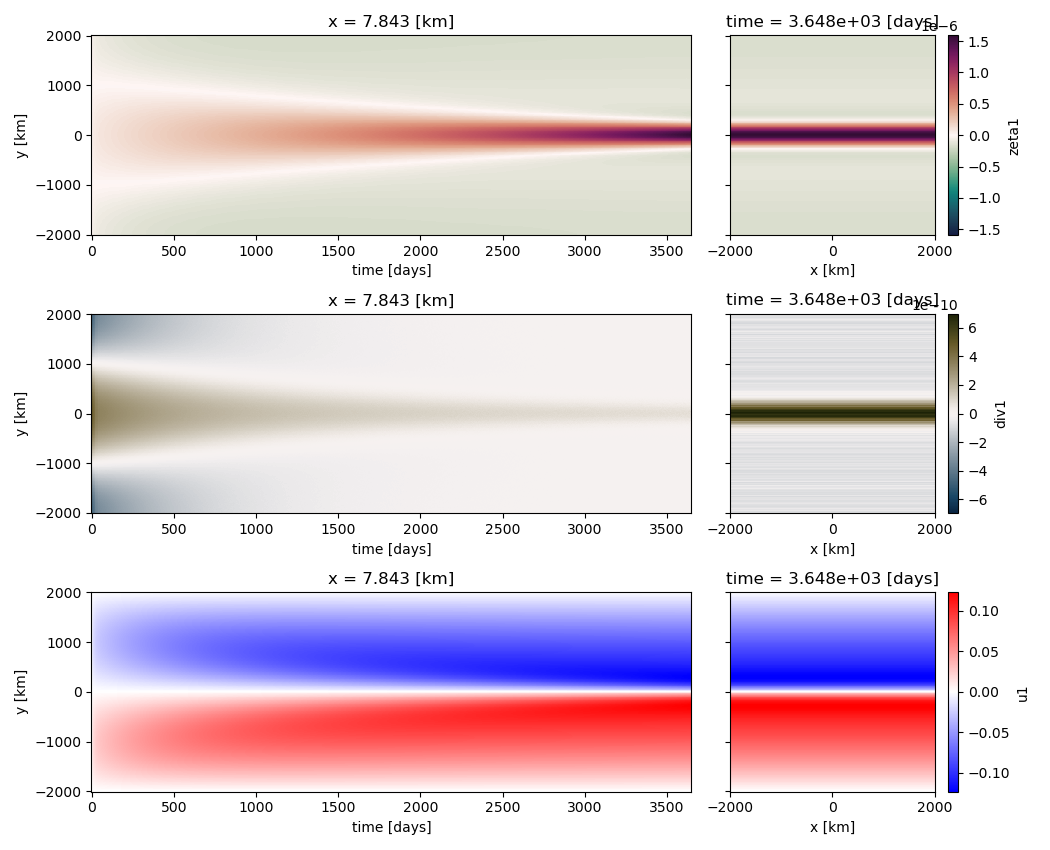
\includegraphics[width=.9\linewidth]{figures/tests/test1_2023-03-31.png}
\caption{\label{fig:orgada75b3}Diagrames de Hovmoler pour les trois couches, période de 10 ans.}
\end{figure}
\begin{figure}[htbp]
\centering
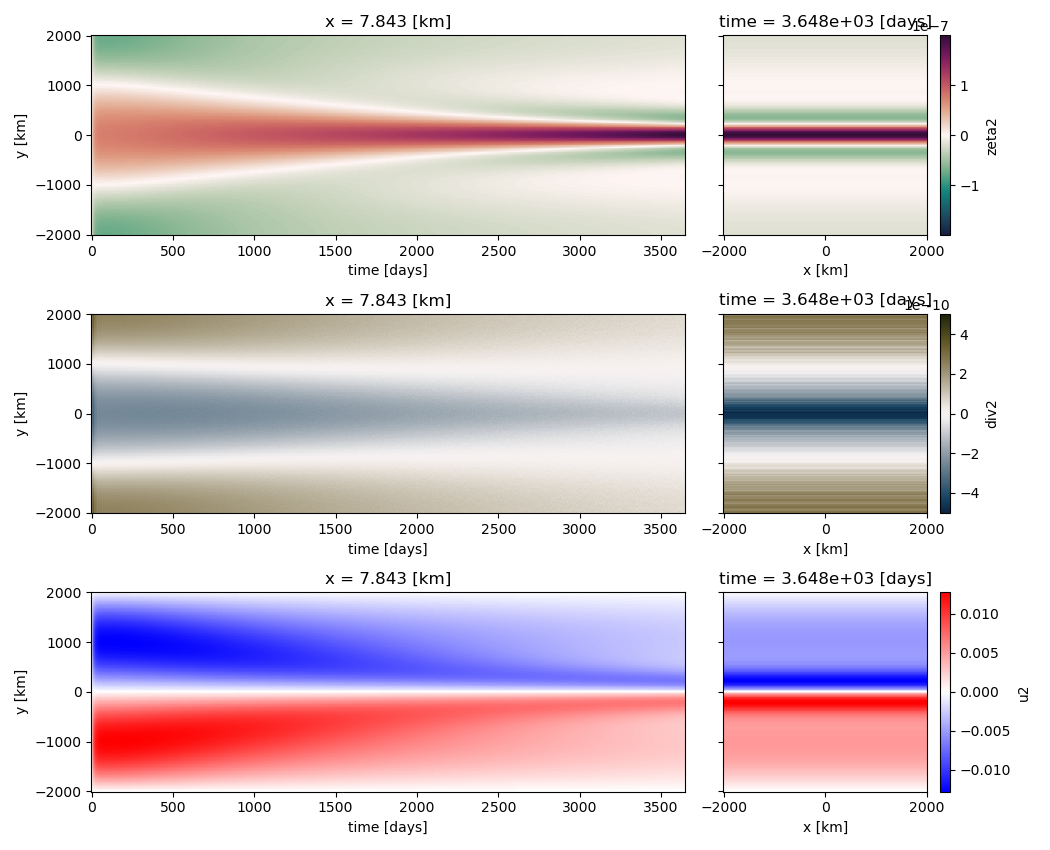
\includegraphics[width=.9\linewidth]{figures/tests/test2_2023-03-31.png}
\caption{\label{fig:orgada75b3}Diagrames de Hovmoler pour les trois couches, période de 10 ans.}
\end{figure}
\begin{figure}[htbp]
\centering
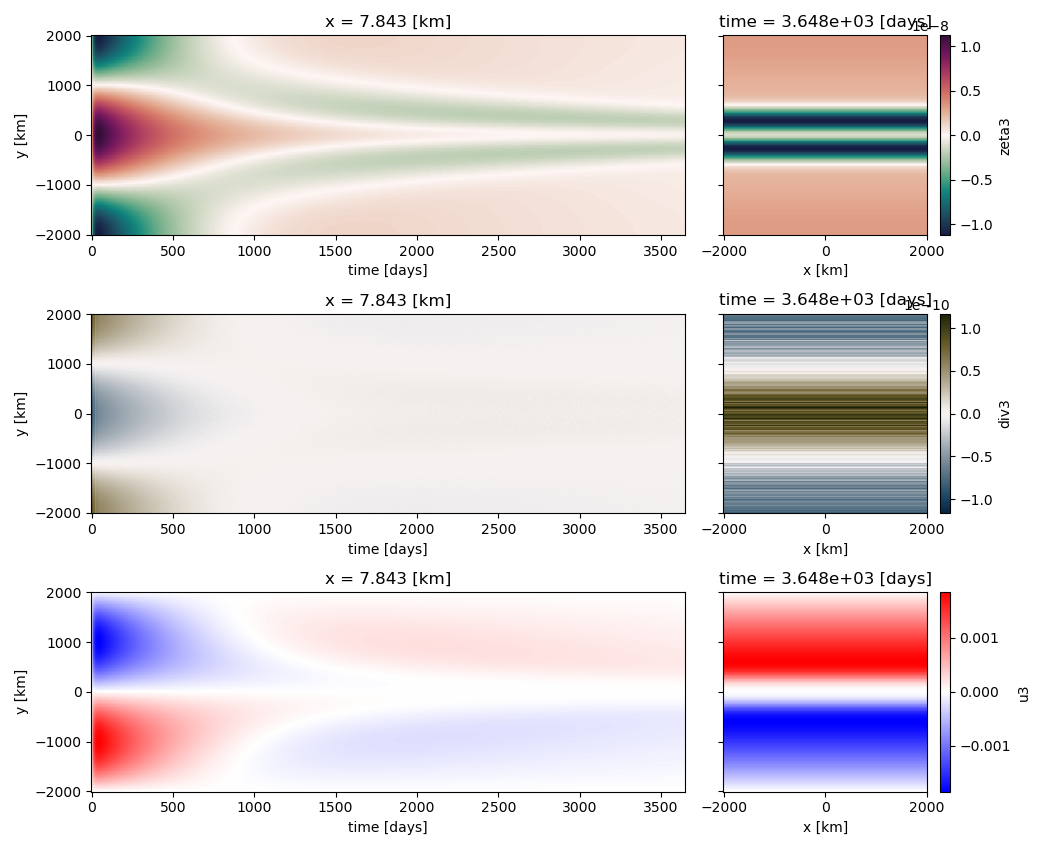
\includegraphics[width=.9\linewidth]{figures/tests/test3_2023-03-31.png}
\caption{\label{fig:orgada75b3}Diagrames de Hovmoler pour les trois couches, période de 10 ans.}
\end{figure}
\end{document}